\section{Stateful Firewall}
Mit der \nameref{sec:proxy-based-firewall} wurde bereits eine erweiterung der einfachen \nameref{sec:packet-filter-firewall} vorgestellt.

Die Stateful Firewall erweitert die \nameref{sec:proxy-based-firewall}. Dabei erhält sie die Möglichkeit, die verarbeitete Kommunikation nicht nur Paketweise zu bewerten und zu klassifizieren, sondern diese auch mit bereits vergangenen Kommunikationsvorgängen in Zusammenhang zu bringen.

\subsection*{Kontext}
Um bessere Sicherheit bspw. gegen Denail of Service \cite{DoS} zu gewährleisten, soll eine zustandslose Firewall die Möglichkeit erhalten, die untersuchten Pakete in einen höheren Zusammenhang bringen zu können.

\subsection*{Problem}
Wie können eingehende Pakete nicht nur einzeln kontrolliert (vgl. \nameref{sec:packet-filter-firewall}) sondern auch miteinander in Verbindung gebracht werden?

Wie kann dieser Sachverhalt weiter dazu verwendet werden, eine höhere Sicherheit zu gewährleisten?


\subsection*{Lösung}
Stellt ein Client eine Verbindung zur Firewall her, wird diese Verbindung in einer Liste/Tabelle zwischengespeichert und als \emph{geöffnet} markiert.

Dies ermöglicht das optimierte überprüfen (oder eben gerade nicht-überprüfen) von weiteren eingehenden Paketen des selben Clients.

\begin{figure}[H]
	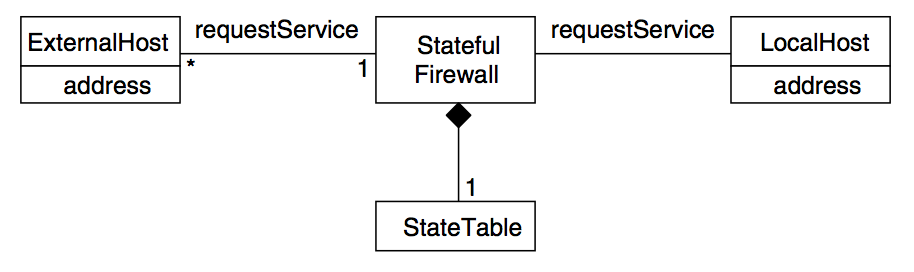
\includegraphics[width=10cm]{content/firewall-architectures/images/stateful-structure.png}
	\caption{Stateful Firewall: Schematischer Aufbau}
\end{figure}

\subsubsection*{Implementierung: Handling eines Requests}
\begin{figure}[H]
	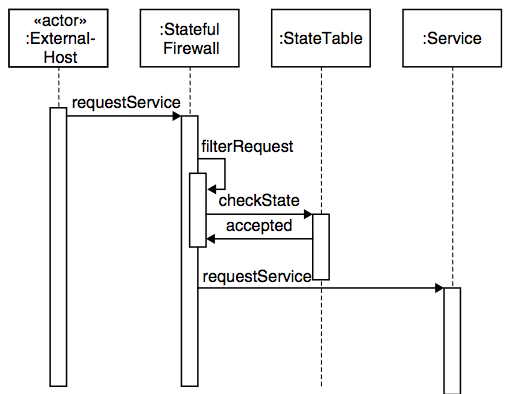
\includegraphics[width=10cm]{content/firewall-architectures/images/stateful-sequence.png}
	\caption{Stateful Firewall: Ablauf \cite{SecPatterns06}}
\end{figure}

\begin{enumerate}
	\item Client (External Host) greift auf das System zu
	\item Die Stateful Firewall prüft, ob die Verbindung zum Client bereits in der State Table vorhanden ist. Sollte dies der Fall sein, wird der Request weitergeleitet.
	\item Existiert die Verbindung noch nicht in der State Table, wird der Request gem. der \nameref{sec:packet-filter-firewall} geprüft. Soll der Request zugelassen werden, wird die Verbindung zum Client in die State Table eingetragen und der Request anschliessend weitergeleitet.
\end{enumerate}

Neben einer Kombination mit einer \nameref{sec:packet-filter-firewall} ist auch eine Verwendung der Stateful Firewall mit der \nameref{sec:proxy-based-firewall} problemlos umsetzbar.

\subsection*{Vorteile}
\begin{itemize}
	\item In der einfachen \nameref{sec:packet-filter-firewall}-Kombination ist die Implementierung relativ kostengünstig und bietet einen guten Schutz
	\item Die Effizienz im Bezug auf den Sicherheitsaspekt der einfacheren Firewall Patterns kann durch die neuen Zustandsinformationen gesteigert werden
	\item Für neue Attacktypen müssen lediglich neue Vergleichsalgorithmen/Regeln implementiert werden
\end{itemize}

\subsection*{Nachteile}
\begin{itemize}
	\item Mit dem Wissen über die Existenz einer State Table kann theoretisch eine Attacke speziell zur Überlastung der Firewall geplant werden
	\item Es können nur Attacken erkannt werden, für welche auch entsprechende Erkennungsalgorithmen vorhanden sind (Firmwareupgrades nötig?)
\end{itemize}

\subsection*{Mögliche Prüfungsfragen}
\begin{itemize}
	\item \emph{Ist eine Stateful Firewall ein eigenständiges Pattern?}\\
	Nein, es erweitert mindestens das \nameref{sec:packet-filter-firewall} Pattern.
\end{itemize}